\documentclass[tikz, border = 1 cm]{standalone}

%%%%%%%%%%%%%%
\usepackage{bm}
\usepackage{tikz}
\usetikzlibrary{calc}
%%%%%%%%%%%%%%

%%%%%%%%%%%%%%
\definecolor{blue4}		{RGB}{178,231,248}
\definecolor{bluegray3}	{RGB}{127,191,211}
\definecolor{gray1}		{RGB}{76,84,93}
\definecolor{gray4}		{RGB}{201,203,206}
\definecolor{orange4}	{RGB}{255,216,192}
%%%%%%%%%%%%%%

%%%%%%%%%%%%%%
%%%%%%%%%%%%%%
%%%%%%%%%%%%%%
\begin{document}

%%%%%%%%%%%%%%
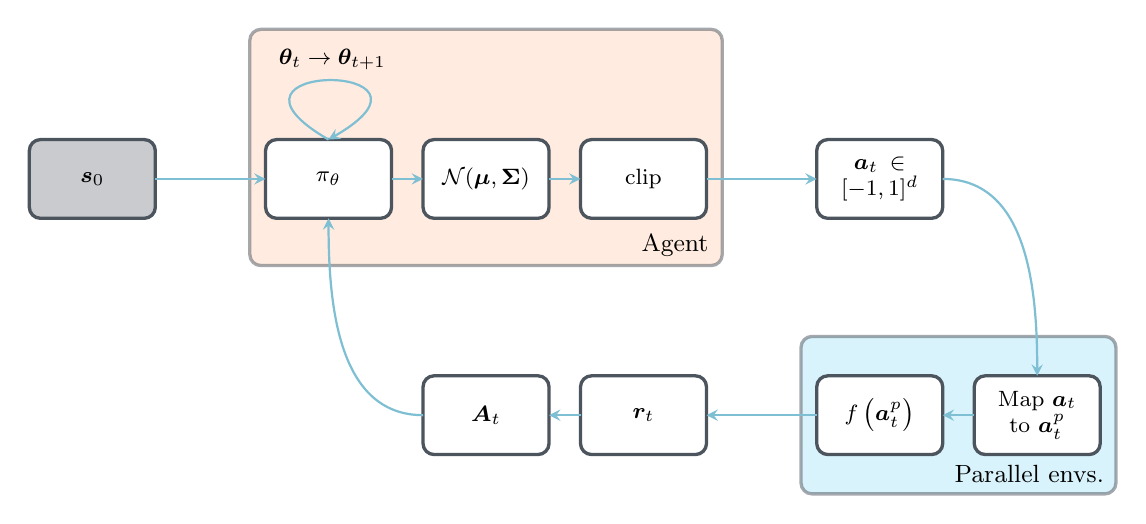
\begin{tikzpicture}[	every loop/.style={	min distance=20mm,looseness=20},
				fontsize/.style={		font=\footnotesize},
				intnode/.style={		black, fontsize, pos=0.5},
				arrow/.style={		thick,color=bluegray3, rounded corners,thick,-stealth},
				box/.style={		rectangle,rounded corners, draw=gray1, very thick, 
								text width=1.6cm,minimum height=1cm,text centered,
								inner sep=0pt, outer sep=0pt, fontsize},
				backbox1/.style={	box, opacity=0.5,text width=6cm,minimum height=3cm},
				backbox2/.style={	box, opacity=0.5,text width=4cm,minimum height=2cm}]

	%% nodes
	\node[box,fill=gray4] 				(s0) 		at (0,0) {$\bm{s}_0$};
	
	\node[backbox1,fill=orange4]		(agent)	at (5,0.4) {};
	\node[xshift=-0.6cm,yshift=0.25cm]	(agt)		at (agent.south east) {\small Agent};
	\node[box,fill=white] 				(nn) 		at (3,0) {$\pi_\theta$};
	\node[box,fill=white] 				(normal) 	at (5,0) {$\mathcal{N}(\bm{\mu},\bm{\Sigma})$};
	\node[box,fill=white] 				(sclip) 	at (7,0) {clip};
	
	\node[box,fill=white] 				(at) 		at (10,0) {$\bm{a}_t \in [-1,1]^{d}$};
	
	\node[backbox2,fill=blue4]			(env)		at (11,-3) {};
	\node[xshift=-1.1cm,yshift=0.25cm]	(evt)		at (env.south east) {\small Parallel envs.};
	\node[box,fill=white] 				(atp) 		at (12,-3) {Map $\bm{a}_t$ to $\bm{a}^p_t$};
	\node[box,fill=white] 				(f) 		at (10,-3) {$f \left( \bm{a}^p_t \right)$};
	
	\node[box,fill=white] 				(rwd) 	at (7,-3) {$\bm{r}_t$};
	\node[box,fill=white] 				(adv) 	at (5,-3) {$\bm{A}_t$};
	
	%% arrows
	\draw[] 		(nn.north) 	edge	[out=150,in=30, loop,arrow] node[intnode, above] {$\,\,\bm{\theta}_t \to \bm{\theta}_{t+1}$} (nn.north);
	
	\draw[arrow] 	(s0) 			to 	[out=0,in=180] 	(nn.west);
	\draw[arrow] 	(nn.east)		to 	[out=0,in=180] 	(normal.west);
	\draw[arrow] 	(normal.east)	to 	[out=0,in=180] 	(sclip.west);
	\draw[arrow] 	(sclip.east)	to 	[out=0,in=180] 	(at.west);
	\draw[arrow] 	(at.east)		to 	[out=0,in=90] 	(atp.north);
	\draw[arrow] 	(atp.west)		to 	[out=180,in=0] 	(f.east);
	\draw[arrow] 	(f.west)		to 	[out=180,in=0] 	(rwd.east);
	\draw[arrow] 	(rwd.west)		to 	[out=180,in=0] 	(adv.east);
	\draw[arrow] 	(adv.west)		to 	[out=180,in=-90] (nn.south);
	
\end{tikzpicture}
%%%%%%%%%%%%%%

\end{document}